\documentclass[11pt]{article}
\usepackage{amsmath} 
\usepackage{graphicx}
\usepackage{subcaption}
\usepackage{sectsty}
\usepackage{amssymb}
 \usepackage{lipsum}
\usepackage{titlesec}
\usepackage{romannum}
\usepackage{enumitem}
\usepackage{mathtools}
\usepackage[super]{nth}
\usepackage{tikz}
\usepackage{listings}
\usepackage{color}
\usepackage{pagecolor,lipsum}

\definecolor{dkgreen}{rgb}{0,0.6,0}
\definecolor{gray}{rgb}{0.5,0.5,0.5}
\definecolor{mauve}{rgb}{0.58,0,0.82}
\pagecolor{white}
\graphicspath{ {./images/} }
\lstset{frame=tb,
  language=Python,
  aboveskip=3mm,
  belowskip=3mm,
  showstringspaces=false,
  columns=flexible,
  basicstyle={\small\ttfamily},
  numbers=none,
  numberstyle=\tiny\color{gray},
  keywordstyle=\color{blue},
  commentstyle=\color{dkgreen},
  stringstyle=\color{mauve},
  breaklines=true,
  breakatwhitespace=true,
  tabsize=3
}

\newcommand*\circled[1]{\tikz[baseline=(char.base)]{
            \node[shape=circle,draw,inner sep=2pt] (char) {#1};}}

\setlist[itemize,1]{leftmargin=\dimexpr 26pt-.5in}

\sectionfont{\fontsize{12}{15}\selectfont}
\title{Introduction to Programming with Python}
\author{Qitian Liao}
\date{Aug 3, 2020} 
\usepackage[left=2cm, right=2cm, top=2cm]{geometry}
\setlength\parindent{0pt}

\DeclarePairedDelimiter\abs{\lvert}{\rvert}
\DeclarePairedDelimiter\norm{\lVert}{\rVert}

\begin{document}
%\pagenumbering{gobble}
\maketitle
\newpage
\tableofcontents
\def\Arg{\mathop{\operator@font Arg}\nolimits}
%\newpage
\pagenumbering{arabic}
\titleformat*{\section}{\Large\bfseries}
\titleformat*{\subsection}{\large\bfseries}
\titleformat*{\subsubsection}{\normalsize\bfseries}
\titleformat*{\paragraph}{\large\bfseries}
\titleformat*{\subparagraph}{\large\bfseries}

\titlespacing\section{0pt}{5pt plus 4pt minus 2pt}{5pt plus 2pt minus 2pt}
\titlespacing\subsection{0pt}{10pt plus 4pt minus 2pt}{5pt plus 2pt minus 2pt}
\titlespacing\subsubsection{0pt}{5pt plus 4pt minus 2pt}{5pt plus 2pt minus 2pt}

\newpage
\section{Functions}
\subsection{Elements of Programming} 
Every programming language has three basic mechanisms: \\
\textbf{Primitive expressions and statements}: This represents the simplest building blocks that the language provides \\
\textbf{Means of combination}: Compound elements are built from simpler ones \\
\textbf{Means of abstraction}: Compound elements can be named and manipulated as units.
\newline
\subsection{Expressions}
An expression describes a computation and evaluates to a value. \\
\textbf{Primitive Expressions}: 
\begin{enumerate}
\item Number or Numeral. 
More precisely, the expression that you type consists of the numerals that represent the number in base 10. Expressions representing numbers may be combined with mathematical operators to form a compound expression, which the interpreter will evaluate. 
\begin{lstlisting}
>>> 13 + 13
26
\end{lstlisting}
These mathematical expressions use infix notation, where the operator (e.g., +, -, *, or /) appears in between the operands (numbers). Python includes many ways to form compound expressions. 
\item Name
\begin{lstlisting}
>>> max
<built-in function max>
\end{lstlisting}
\item String 
\begin{lstlisting}
>>> "about" 
'about'
\end{lstlisting} 
\end{enumerate}


\subsection{Call Expressions}
The most important kind of compound expression is a call expression, which applies a function to some arguments. 
\begin{lstlisting}
>>> max(6, 8) 
8
\end{lstlisting}
$$\mbox{Operator}(\mbox{Operand}, \mbox{Operand})$$
This call expression has subexpressions: the operator is an expression that precedes parentheses, which enclose a comma-delimited list of operand expressions. The operator specifies a function. When this call expression is evaluated, the function max is called with arguments 6 and 8, and returns a value of 8. \\
\newline
\textbf{Evaluation procedure for call expressions}
\begin{enumerate}
\item Evaluate the operator and then the operand subexpressions. 
\item Apply the function that is the value of the operator subexpression to the arguments that are the values of the operand subexpression. 
\end{enumerate} 
The order of the arguments in a call expression matters. For instance, the function pow raises its first argument to the power of its second argument. 
\begin{lstlisting}
>>> pow(2, 5) 
32 
>>> pow(5, 2) 
25
\end{lstlisting}
Function notation has three principal advantages over the mathematical convention of infix notation. \\
\begin{enumerate} 
\item Functions may take an arbitrary number of arguments. 
\begin{lstlisting}
>>> max(1, 2, 3, 4)
4
\end{lstlisting} 
\item Function notation extends in a straightforward way to nested expressions, where the elements are themselves compound expressions. In nested call expressions, unlike compound infix expressions, the structure of the nesting is entirely explicit in the parentheses. 
\begin{lstlisting}
>>> max(min(1, -2), min(pow(3, 5), -4))
-2
\end{lstlisting}
\item Mathematical notation has a great variety of forms: multiplication appears between terms, exponents appear as superscripts, division as a horizontal bar, and a square root as a roof with slanted siding. All of this complexity can be unified via the notation of call expressions. While Python supports common mathematical operators using infix notation (like + and -), any operator can be expressed as a function with a name.
\end{enumerate}

\subsection{Importing Library Functions}
Python defines a very large number of functions, including the operator functions mentioned in the preceding section, but does not make all of their names available by default. Instead, it organizes the functions and other quantities that it knows about into modules, which together comprise the Python Library. To use these elements, one imports them. \\
For example, the math module provides a variety of familiar mathematical functions:
\begin{lstlisting}
from math import sqrt
>>> sqrt(25) 
5
\end{lstlisting}

The operator module provides access to functions corresponding to infix operators: 

\begin{lstlisting} 
from operator import add, sub, mul
>>> add(3, 5)
8
\end{lstlisting}
An import statement designates a module name (e.g., math), and then lists the named attributes of that module to import (e.g., sqrt). Once a function is imported, it can be called multiple times. \\
There is no difference between using these operator functions (e.g., add) and the operator symbols themselves (e.g., +). Conventionally, most programmers use symbols and infix notation to express simple arithmetic.

\subsection{Exercises} 
Evaluate the following equations: 
\begin{lstlisting}
>>> max(min(3, -2), min(pow(2, 5), -4))
\end{lstlisting}

\newpage
\section{Names, Assignment and User-Defined Functions}
\subsection{Names} 
A critical aspect of a programming language is the means it provides for using names to refer to computational objects. If a value has been given a name, we say that the name binds to the value. 
\subsection{Assignment}
In Python, we can establish new bindings using the assignment statement, which contains a name to the left of = and a value to the right: 
\begin{lstlisting}
>>> a = 10 
>>> a 
10 
>>> a + 2
12 
\end{lstlisting}
The = symbol is called the assignment operator in Python. Assignment is our simplest means of abstraction, for it allows us to use simple names to refer to the results of compound operations. In this way, complex programs are constructed by building, step by step, computational objects of increasing complexity. \\ 
\textbf{Environment}: 
The possibility of binding names to values and later retrieving those values by name means that the interpreter must maintain some sort of memory that keeps track of the names, values, and bindings. This memory is called an environment. \\
\newline
Names can also be bound to functions. For instance, the name max is bound to the max function we have been using. Functions, unlike numbers, are tricky to render as text, so Python prints an identifying description instead, when asked to describe a function. 
\begin{lstlisting}
 >>> max 
 <built-in function max>
\end{lstlisting}
We can use assignment statements to give new names to existing functions.
\begin{lstlisting}
 >>> f = max
 >>> f 
 <built-in function max>
 >>> f(1, 2, 3) 
 3
\end{lstlisting}
And successive assignment statements can rebind a name to a new value. 
\begin{lstlisting}
>>> f = 2
>>> f
2 
\end{lstlisting} 
In Python, names are often called variable names or variables because they can be bound to different values in the course of executing a program. When a name is bound to a new value through assignment, it is no longer bound to any previous value. One can even bind built-in names to new values. 
\begin{lstlisting} 
>>> max = 5
>>> max 
5
\end{lstlisting} 
After assigning max to 5, the name max is no longer bound to a function, and so attempting to call max(2, 3, 4) will cause an error. 
\begin{lstlisting}
>>> max(1, 2)
Traceback (most recent call last):
File "<stdin>", line 1, in <module>
TypeError: 'int' object is not callable 
\end{lstlisting}
When executing an assignment statement, Python evaluates the expression to the right of = before changing the binding to the name on the left. Therefore, one can refer to a name in right-side expression, even if it is the name to be bound by the assignment statement. 
\begin{lstlisting}
>>> x = 2
>>> x = x + 1
>>> x 
3
\end{lstlisting} 
We can also assign multiple values to multiple names in a single statement, where names on the left of = and expressions on the right of = are separated by commas. 
\begin{lstlisting}
>>> a, b = 1, 2
>>> a 
1 
>>> b
2
\end{lstlisting}
With multiple assignment, all expressions to the right of = are evaluated before any names to the left are bound to those values. As a result of this rule, swapping the values bound to two names can be performed in a single statement.
\begin{lstlisting}
>>> a, b = 1, 2
>>> a, b = b, a
>>> a 
2
>>> b
1
\end{lstlisting} 
\subsection{The Non-pure Print Function} 
The special \textbf{None} represents nothing in Python. A function that does not explicitly return a value will return \textbf{None}. \textbf{None} is not displayed by the interpreter as the value of an expression. \\
\newline
\textbf{Pure functions}: Functions have some input (their arguments) and return some output (the result of applying them). The built-in function abs can be depicted as a small machine that takes input and produces output. From the output below, we can see that the function \textbf{abs} is pure.
\begin{lstlisting}
>>> abs(-1)
1 
\end{lstlisting} 
Properties of pure functions: 
\begin{enumerate}
\item Applying them has no effects beyond returning a value. 
\item Must always return the same value when called twice with the same arguments.
\end{enumerate}
\textbf{Non-pure functions}: In addition to returning a value, applying a non-pure function can generate side effects, which make some change to the state of the interpreter or computer. A common side effect is to generate additional output beyond the return value, using the \textbf{print} function. 
\begin{lstlisting}
>>> print(1, 2, 3)
1 2 3
\end{lstlisting}
While \textbf{print} and \textbf{abs} may appear to be similar in these examples, they work in fundamentally different ways. The value that \textbf{print} returns is always \textbf{None}.The interactive Python interpreter does not automatically print the value \textbf{None}. In the case of print, the function itself is printing output as a side effect of being called. \\
A nested expression of calls to print highlights the non-pure character of the function. 
\begin{lstlisting}
>>> print(print(1), print(2))
1
2 
None None
\end{lstlisting}
Let us see another example. 
\begin{lstlisting}
>>> two = print(2)
2
>>> print(two)
None 
\end{lstlisting} 
\subsection{Exercises}
For each of the expressions below, write the output displayed by the interactive Python interpreter when the expression is evaluated. The output may have multiple lines. If an error occurs, write "Error", but include all output displayed before the error. If a function is displayed, write "Function". \\
Recall: The interactive interpreter displays the value of a successfully evaluated expression, unless it is \textbf{None}. 
\begin{lstlisting}
>>> print(1, print(2))
\end{lstlisting}
\begin{lstlisting}
>>> print(None, print(None))
\end{lstlisting}
\begin{lstlisting}
>>> print(print(print(2)), print(3))
\end{lstlisting}
\begin{lstlisting}
>>> print(4, 5) + 1
\end{lstlisting}

\newpage
\section{Control}
\subsection{Defining Functions} 
Function definition is a more powerful means of abstraction, in which it binds names to expressions. 
\begin{lstlisting}
def <name>(<formal parameters>):
	return <return expression>
\end{lstlisting} 
Execution procedure for def statements: 
\begin{enumerate}
\item Create a function with signature $<$name$>$($<$formal parameters$>$). Function signature indicates how many arguments a function takes. 
\item Set the body of that function to be everything indented after the first line. Function body defines the computation performed when the function is applied. 
\item Bind $<$name$>$ to that function in the current frame. 
\end{enumerate} 
\subsubsection{Environmental Diagrams} 
\begin{enumerate}
\item Every expression is evaluated in the context of an environment. Names have no meaning without an environment. 
\item An environment is a sequence of frames, starting with the global frame and followed by a sequence of local frames.
\item A name evaluates to the value bound to that name in the earliest frame of the current environment in which that name is found. 
\end{enumerate}
Look at the following example. 
\begin{lstlisting}
>>> from operator import mul
>>> def square(x):
		return mul(x, x)
>>> square(square(3))
\end{lstlisting} 
The corresponding environmental diagram is on the next page. \\
\begin{figure}[h]
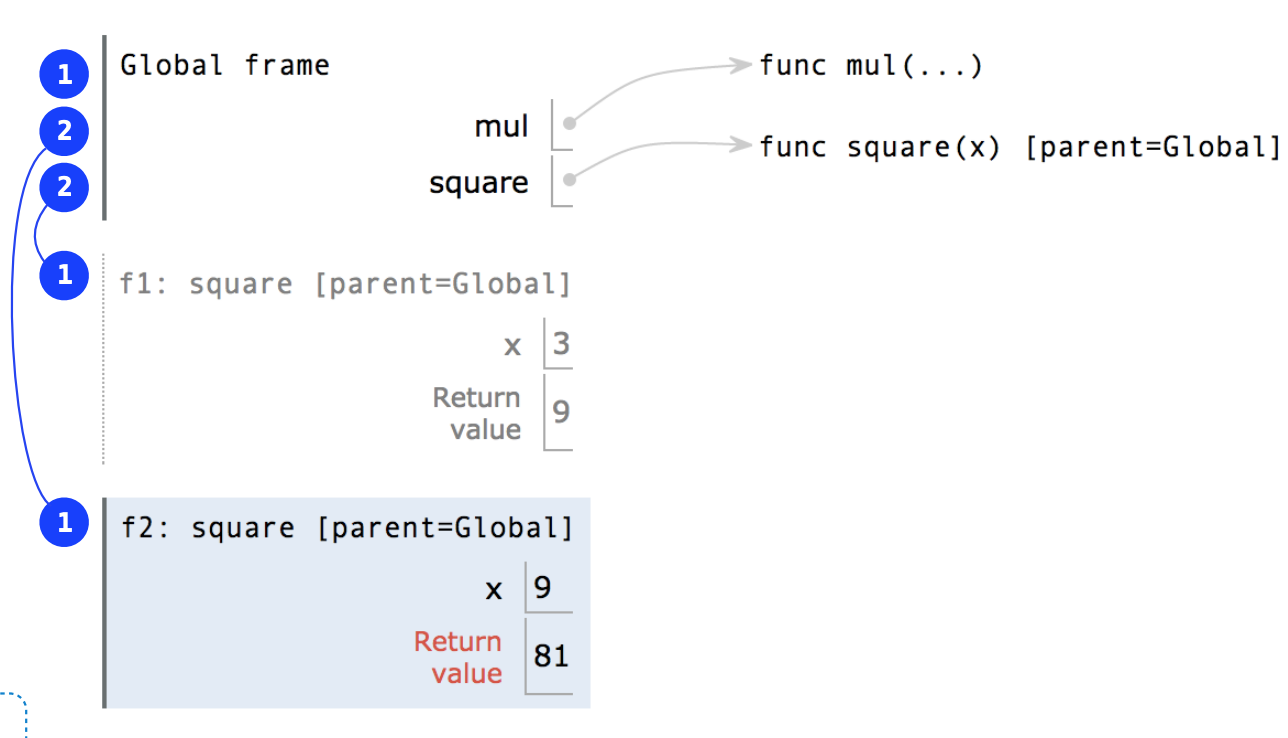
\includegraphics[scale=0.7]{Lec3} 
\centering
\end{figure}
\newline
Sometimes we will have very complicated function calls, and environmental diagrams will come in very handy at that time. Look at the following example. (credit to CS61A Midterm Spring 2015). We will try to solve this after we cover higher order functions. 
\begin{lstlisting}
batman, superman, ivy = 1, -2, -3 
def nanana(batman):
	while batman(superman) > ivy: 
		def batman(joker):
			return ivy
	return -ivy

def joker(superman):
	if superman(batman):
		ivy = -batman
	return nanana
	
joker(abs)(abs)
\end{lstlisting}

\subsubsection{Life Cycle of a User-Defined Function}
\begin{enumerate}
\item Def Statement: A new function is created. Name bound to that function is in the current frame.
\item Call Expression: Operator and operands are evaluated. Function (value of operator) called on arguments (value of operands).
\item Calling/Applying: A new frame is created. Parameters are bound to the arguments. Body is executed in that new environment.
\end{enumerate}

\subsection{Conditional Statement}
A statement is executed by the interpreter to perform an action. 
\subsubsection{Compound Statements} 
Above we have seen how we can define functions. And def statements are compound statements. 
\begin{lstlisting} 
>>> <header>: 
>>> 		<statement> 
>>> 		<statement>
>>> 		...
>>> <seperating header> 
>>> 		<statement>
>>> 		<statement>
>>> 		...
\end{lstlisting}
The first header determines a statement's type. The header of a clause controls the suite that follows. \\
A suite is a sequence of statements. To execute a suite means to execute its sequence of statements, in order. \\
Execution Rule for a sequence of statements: 
\begin{enumerate}
\item Execute the first statement.
\item Unless directed otherwise, execute the rest. 
\end{enumerate} 
\subsubsection{Conditional Statements}
We start with the following example with 1 statement, 3 clauses, 3 headers, and 3 suites. 
\begin{figure}[h]
\includegraphics[scale=1]{statement} 
\centering
\end{figure}
\begin{lstlisting}
>>> def abs(x): 
...     if x < 0: 
...             return -x
...     elif x == 0:
...             return 0
...     else:
...             return x
\end{lstlisting}
\textbf{Execution Rule for Conditional Statements:} \\
Each clause is considered in order. 
\begin{enumerate}
\item Evaluate the header's expression. 
\item If it is a true value, execute the suite and skip the remaining clauses.
\end{enumerate}
\textbf{Syntax Tips:}
\begin{enumerate}
\item Always starts with "if" clause. 
\item Zero or more "elif" clauses. 
\item Zero or one "else" clause, always at the end.  
\end{enumerate}
\subsection{Boolean Contexts and Operators}
Python supports three boolean operators: \textbf{and}, \textbf{or}, and \textbf{not}. 
\begin{lstlisting}
>>> a = 4
>>> a < 2 and a > 0
False
>>> a < 2 or a > 0 
True 
>>> not (a > 0) 
False
\end{lstlisting}
\begin{enumerate}
\item \textbf{and} evaluates to \textbf{True} only if both operands evaluate to \textbf{True}. If at least one operand is \textbf{False}, then and evaluates to \textbf{False}.
\item \textbf{or} evaluates to \textbf{True} if at least one operand evaluates to \textbf{True}. If both operands are \textbf{False}, then or evaluates to \textbf{False}.
\item \textbf{not} evaluates to \textbf{True} if its operand evaluates to \textbf{False}. It evaluates to \textbf{False} if its operand evalutes to \textbf{True}.
\end{enumerate}
Let us look at a more complicated example. 
\begin{lstlisting}
>>> (True and (not False)) or ((not True) and False) 
\end{lstlisting}
Before we can solve this, we need to know that boolean operators have an order of operation: \\
\textbf{not} have the highest priority, then \textbf{and}, lastly \textbf{or} has the lowest priority. Let us try again. \\ 
\subsubsection{Short Circuiting}
First, let us look at the example below. 
\begin{lstlisting}
>>> 1 / 0
Traceback (most recent call last):
  File "<stdin>", line 1, in <module>
ZeroDivisionError: division by zero
>>> True or 1/0
True
\end{lstlisting}
The behavior is curious. The second expression evaluates to \textbf{True} because Python's \textbf{and} and \textbf{or} operators short-circuit. That means they do not necessarily evaluate every operand. \\
Short-circuiting happens when the operator reaches an operand that allows them to make a conclusion about the expression. For example, \textbf{and} will short-circuit as soon as it reaches the first false value because it then knows that not all the values are true. \\
If \textbf{and} and \textbf{or} do not short-circuit, they just return the last value. Keep in mind that \textbf{and} and \textbf{or} don't always return booleans when using values other than \textbf{True} and \textbf{False}.
\begin{figure}[h]
\includegraphics[scale=0.5]{boolean} 
\centering
\end{figure}
\newline
\newline
False values in Python: False, 0, '', None (more to come) \\
True values in Python: Anything else. 

\subsection{Division}
\begin{figure}[h]
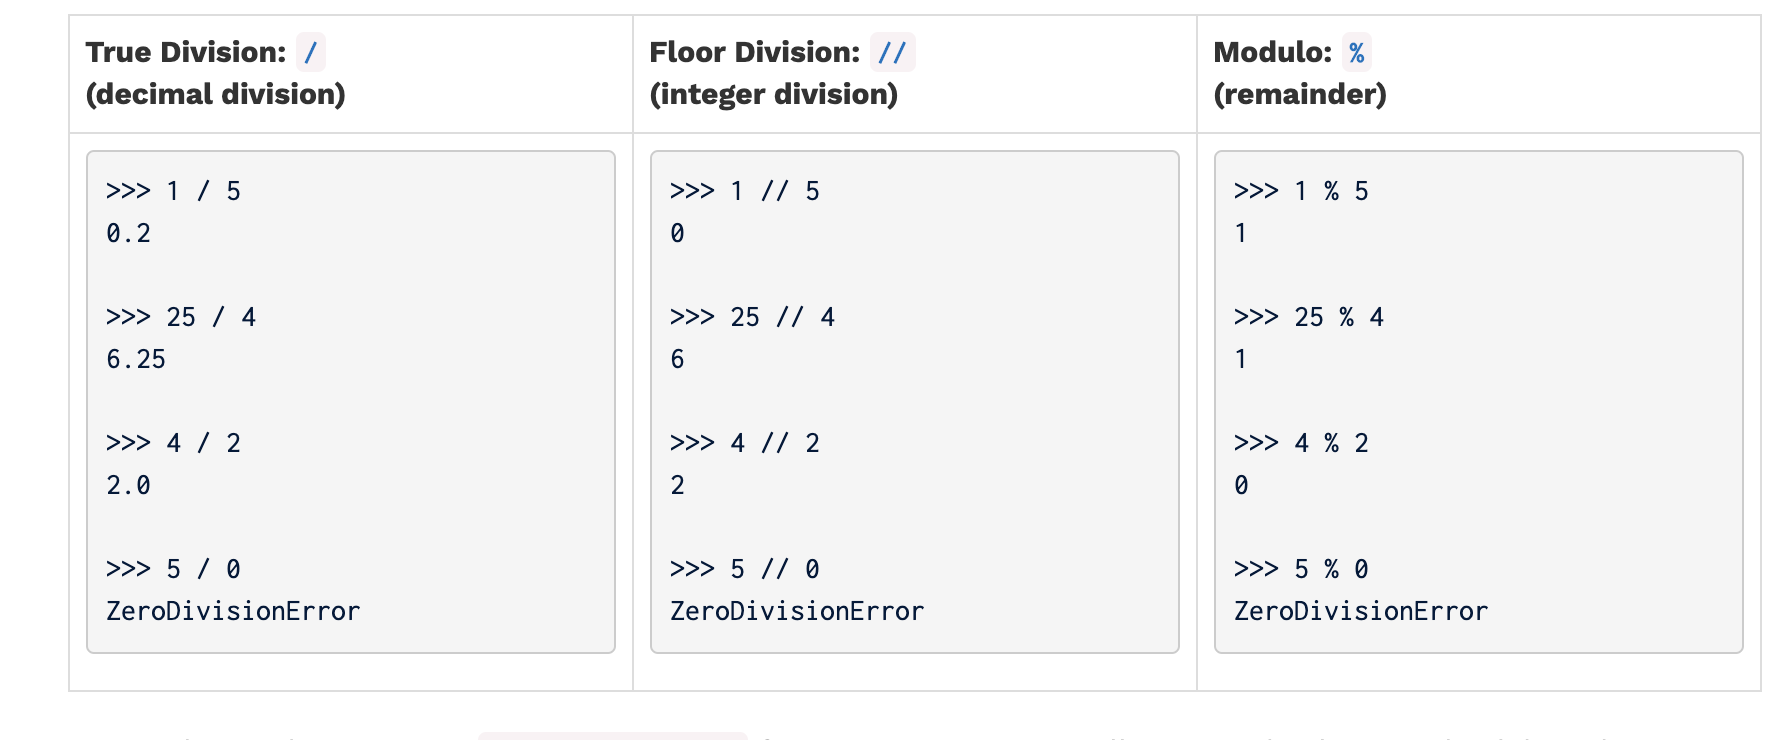
\includegraphics[scale=0.6]{Division} 
\centering
\end{figure}

\iffalse
\subsection{Iteration}
\subsubsection{While Statements} 
\textbf{Execution Rule for While Statements:} 
\begin{enumerate}
\item Evaluate the header's expression.
\item If it is a true value, execute the (whole) suite, then return to step 1. 
\end{enumerate}
\fi

\subsection{Exercises}
\begin{enumerate}[leftmargin = *]
\item
\begin{lstlisting}
>>> True and 13
______

>>> False or 0
______

>>> not 10
______

>>> not None
______
>>> True and 1 / 0 and False
______

>>> True or 1 / 0 or False
______

>>> True and 0
______

>>> False or 1
______

>>> 1 and 3 and 6 and 10 and 15
______

>>> 0 or False or 2 or 1 / 0
______
>>> not 0
______

>>> (1 + 1) and 1
______

>>> 1/0 or True
______

>>> (True or False) and False
______

\end{lstlisting}
\item Write a function that takes three positive numbers and returns the sum of the squares of the two largest numbers. \\
\textbf{Challenge:} Use only a single line for the body of the function.  
\begin{lstlisting}
def two_of_three(a, b, c):
    """Return x*x + y*y, where x and y are the two largest members of the positive numbers a, b, and c.
    >>> two_of_three(1, 2, 3)
    13
    >>> two_of_three(5, 3, 1)
    34
    >>> two_of_three(10, 2, 8)
    164
    >>> two_of_three(5, 5, 5)
    50
    """
    return _____
\end{lstlisting}
\item Write a function that takes an integer $n$ that is \textbf{greater than 1} and returns the largest integer that is smaller than $n$ and evenly divides $n$. 
\begin{lstlisting}
def largest_factor(n):
    """Return the largest factor of n that is smaller than n.

    >>> largest_factor(15) # factors are 1, 3, 5
    5
    >>> largest_factor(80) # factors are 1, 2, 4, 5, 8, 10, 16, 20, 40
    40
    >>> largest_factor(13) # factor is 1 since 13 is prime
    1
    """
    "*** YOUR CODE HERE ***"
\end{lstlisting}
Hint: To check if b evenly divides a, you can use the expression a \% b == 0, which can be read as, "the remainder of dividing a by b is 0."
\item Douglas Hofstadter's Pulitzer-prize-winning book, Gödel, Escher, Bach, poses the following mathematical puzzle. \\
\newline
1. Pick a positive integer n as the start. \\
2. If n is even, divide it by 2. \\
3. If n is odd, multiply it by 3 and add 1. \\
4. Continue this process until n is 1. \\
\newline
The number n will travel up and down but eventually end at 1 (at least for all numbers that have ever been tried -- nobody has ever proved that the sequence will terminate). Analogously, a hailstone travels up and down in the atmosphere before eventually landing on earth. \\
\newline
This sequence of values of n is often called a Hailstone sequence, Write a function that takes a single argument with formal parameter name n, prints out the hailstone sequence starting at n, and returns the number of steps in the sequence. 
\begin{lstlisting}
def hailstone(n):
    """Print the hailstone sequence starting at n and return its
    length.

    >>> a = hailstone(10)
    10
    5
    16
    8
    4
    2
    1
    >>> a
    7
    """
    "*** YOUR CODE HERE ***" 
\end{lstlisting}
\item Write a function that takes in a nonnegative integer and sums its digits. (Using floor division and modulo might be helpful here!)
\begin{lstlisting}
def sum_digits(n):
    """Sum all the digits of n.

    >>> sum_digits(10) # 1 + 0 = 1
    1
    >>> sum_digits(4224) # 4 + 2 + 2 + 4 = 12
    12
    >>> sum_digits(1234567890)
    45
    """
    "*** YOUR CODE HERE ***"
\end{lstlisting}
\item Write a function that takes in a number and determines if the digits contain two adjacent 8s.
\begin{lstlisting}
def double_eights(n):
    """Return true if n has two eights in a row.
    >>> double_eights(8)
    False
    >>> double_eights(88)
    True
    >>> double_eights(2882)
    True
    >>> double_eights(880088)
    True
    >>> double_eights(12345)
    False
    >>> double_eights(80808080)
    False
    """
    "*** YOUR CODE HERE ***"
\end{lstlisting}
\item Let's write a function falling, which is a "falling" factorial that takes two arguments, n and k, and returns the product of k consecutive numbers, starting from n and working downwards.
\begin{lstlisting}
def falling(n, k):
    """Compute the falling factorial of n to depth k.

    >>> falling(6, 3)  # 6 * 5 * 4
    120
    >>> falling(4, 0)
    1
    >>> falling(4, 3)  # 4 * 3 * 2
    24
    >>> falling(4, 1)  # 4
    4
    """
    "*** YOUR CODE HERE ***"
\end{lstlisting}
\end{enumerate}

\newpage
\section{Higher Order Functions}
\subsection{Designing Functions}
A function's \textit{domain} is the set of all inputs it might possibly take as arguments. \\
A function's \textit{range} is the set of output values it might possibly return. \\
A pure function's \textit{behavior} is the relationship it creates between input and output. 
\subsection{Locally Defined Functions} 
Functions defined within other function bodies are bound to names in a local frame. Look at the following example. 
\begin{lstlisting}
def make_adder(n): 
"""Return a function that takes one argument k and returns k + n.
>>> add_three = make_adder(3)
>>> add_three(4)
7
"""
	def adder(k):
		return k + n
	return adder
\end{lstlisting} 
Here \textit{make\_adder} is a function that returns another function. \\ 
The name \textit{add\_three} is bound to a function. \\ 
\textit{adder} is a def statement within another def statement. \\
\textit{adder} can refer to names in the enclosing function. 
\subsection{Lambda Expressions} 
So far, each time we have wanted to define a new function, we needed to give it a name. But for other types of expressions, we do not need to associate intermediate values with a name. That is, we can compute $a*b + c*d$ without having to name the subexpressions $a*b$ or $c*d$, or the full expression. In Python, we can create function values on the fly using lambda expressions, which evaluate to unnamed functions. A lambda expression evaluates to a function that has a single return expression as its body. Assignment and control statements are not allowed. Lambda functions are not common in Python, but they are important in general. \\
\newline
We can understand the structure of a lambda expression by constructing a corresponding English sentence: 
$$\underbrace{\text{lambda}}_{\text{A function that }} \underbrace{x}_{\text{ takes } x} \underbrace{:}_{\text{ and returns }} \underbrace{f(g(x))}_{ f(g(x)) }$$
It is important that lambda functions do not have "return" keywords and it must return a single expression. 
\begin{lstlisting}
>>> square = lambda x: x * x
>>> square(4)
16
\end{lstlisting} 
\newpage
\textbf{Lambda Expressions Versus Def Statements.} 
\begin{lstlisting}
>>> square = lambda x: x * x
>>> def square(x):
		return x * x	
\end{lstlisting}
\begin{enumerate}[leftmargin = *]
\item Both create a function with the same domain, range, and behavior.
\item Both bind that function to the name square. 
\item Only the def statement gives the function an intrinsic name, which shows up inenvironment diagrams but doesn't affect execution (unless the function is printed).
\end{enumerate}
\begin{figure}[h]
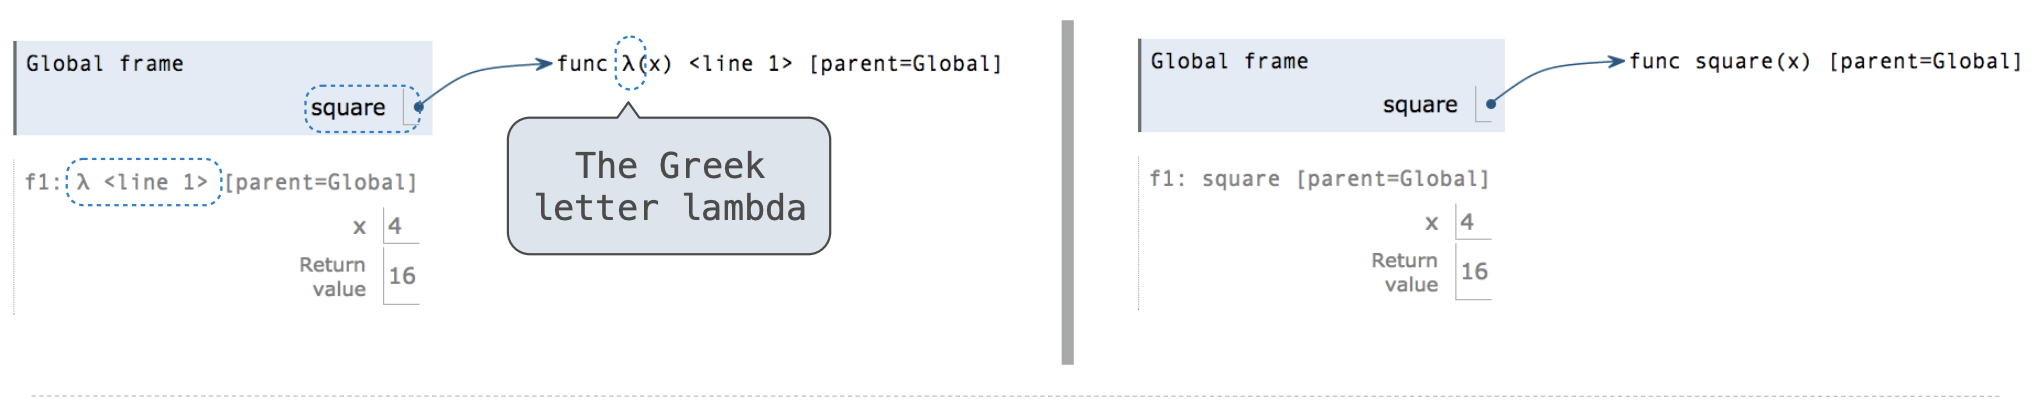
\includegraphics[scale=0.5]{4_1} 
\centering
\end{figure}
\subsection{Exercises}
\begin{enumerate}[leftmargin = *]
\item 
\begin{lstlisting}
>>> lambda x: x  # A lambda expression with one parameter x
______

>>> a = lambda x: x  # Assigning the lambda function to the name a
>>> a(5)
______

>>> (lambda: 3)()  # Using a lambda expression as an operator in a call exp.
______

>>> b = lambda x: lambda: x  # Lambdas can return other lambdas!
>>> c = b(88)
>>> c
______

>>> c()
______

>>> d = lambda f: f(4)  # They can have functions as arguments as well.
>>> def square(x):
...     return x * x
>>> d(square)
______
\end{lstlisting}
\newpage
\item 
\begin{lstlisting}
>>> z = 3
>>> e = lambda x: lambda y: lambda: x + y + z
>>> e(0)(1)()
______

>>> f = lambda z: x + z
>>> f(3)
______
\end{lstlisting}

\item 
\begin{lstlisting}
>>> higher_order_lambda = lambda f: lambda x: f(x)
>>> g = lambda x: x * x
>>> higher_order_lambda(2)(g)  # Which argument belongs to which function call?
______

>>> higher_order_lambda(g)(2)
______

>>> call_thrice = lambda f: lambda x: f(f(f(x)))
>>> call_thrice(lambda y: y + 1)(0)
______

>>> print_lambda = lambda z: print(z)  # When is the return expression of a lambda expression executed?
>>> print_lambda
______

>>> one_thousand = print_lambda(1000)
______

>>> one_thousand
______

\end{lstlisting}

\item
\begin{lstlisting}
>>> def even(f):
...     def odd(x):
...         if x < 0:
...             return f(-x)
...         return f(x)
...     return odd
>>> steven = lambda x: x
>>> stewart = even(steven)
>>> stewart
______

>>> stewart(61)
______

>>> stewart(-4)
______
\end{lstlisting}
\newpage
\item
\begin{lstlisting}
>>> def cake():
...    print('beets')
...    def pie():
...        print('sweets')
...        return 'cake'
...    return pie
>>> chocolate = cake()
______

>>> chocolate
______

>>> chocolate()
______

>>> more_chocolate, more_cake = chocolate(), cake
______

>>> more_chocolate
______

>>> def snake(x, y):
...    if cake == more_cake:
...        return lambda y: x + y
...    else:
...        return x + y
>>> snake(10, 20)
______

>>> snake(10, 20)(30)
______

>>> cake = 'cake'
>>> snake(10, 20)
______

\end{lstlisting}
\newpage
\item
Lambdas and Currying: We can transform multiple-argument functions into a chain of single-argument, higher order functions by taking advantage of lambda expressions. This is useful when dealing with functions that take only single-argument functions. Write a function \textit{lambda\_curry2} that will curry any two argument function using lambdas. 
\begin{lstlisting}
def lambda_curry2(func):
    """
    Returns a Curried version of a two-argument function FUNC.
    >>> from operator import add
    >>> curried_add = lambda_curry2(add)
    >>> add_three = curried_add(3)
    >>> add_three(5)
    8
    """
    "*** YOUR CODE HERE ***"
    return ______
\end{lstlisting}

\item Make Adder with a Lambda: Implement the \textit{make\_adder} function below using a single return statement that returns the value of a lambda expression.
\begin{lstlisting}
def make_adder(n):
    """Return a function that takes an argument K and returns N + K.

    >>> add_three = make_adder(3)
    >>> add_three(1) + add_three(2)
    9
    >>> make_adder(1)(2)
    3
    """
    "*** YOUR CODE HERE ***"
    return 'REPLACE ME'
\end{lstlisting}
\newpage
\item Composite Identity Function: Write a function that takes in two single-argument functions, $f$ and $g$, and returns another function that has a single parameter $x$. The returned function should return True if $f(g(x))$ is equal to $g(f(x))$. You can assume the output of $g(x)$ is a valid input for $f$ and vice versa. You may use the \textit{compose1} function defined below.
\begin{lstlisting}
def compose1(f, g):
    """Return the composition function which given x, computes f(g(x)).

    >>> add_one = lambda x: x + 1        # adds one to x
    >>> square = lambda x: x**2
    >>> a1 = compose1(square, add_one)   # (x + 1)^2
    >>> a1(4)
    25
    >>> mul_three = lambda x: x * 3      # multiplies 3 to x
    >>> a2 = compose1(mul_three, a1)    # ((x + 1)^2) * 3
    >>> a2(4)
    75
    >>> a2(5)
    108
    """
    return lambda x: f(g(x))

def composite_identity(f, g):
    """
    Return a function with one parameter x that returns True if f(g(x)) is
    equal to g(f(x)). You can assume the result of g(x) is a valid input for f
    and vice versa.

    >>> add_one = lambda x: x + 1        # adds one to x
    >>> square = lambda x: x**2
    >>> b1 = composite_identity(square, add_one)
    >>> b1(0)                            # (0 + 1)^2 == 0^2 + 1
    True
    >>> b1(4)                            # (4 + 1)^2 != 4^2 + 1
    False
    """
    "*** YOUR CODE HERE ***"
\end{lstlisting}
\newpage
\item 
Define a function cycle that takes in three functions $f_1$, $f_2$, $f_3$, as arguments. cycle will return another function that should take in an integer argument $n$ and return another function. That final function should take in an argument $x$ and cycle through applying $f_1$, $f_2$, and $f_3$ to $x$, depending on what $n$ was. Here's what the final function should do to $x$ for a few values of $n$:\\
$n = 0$, return $x$ \\
$n = 1$, apply $f_1$ to $x$, or return $f_1(x)$ \\
$n = 2$, apply $f_1$ to $x$ and then $f_2$ to the result of that, or return $f_2(f_1(x))$ \\
$n = 3$, apply $f_1$ to $x$, $f_2$ to the result of applying $f_1$, and then $f_3$ to the result of applying $f_2$, or $f_3(f_2(f_1(x)))$ \\ 
$n = 4$, start the cycle again applying $f_1$, then $f_2$, then $f_3$, then $f_1$ again, or $f_1(f_3(f_2(f_1(x))))$ \\ 
And so forth.\\
Hint: most of the work goes inside the most nested function.
\begin{lstlisting}
def cycle(f1, f2, f3):
    """Returns a function that is itself a higher-order function.

    >>> def add1(x):
    ...     return x + 1
    >>> def times2(x):
    ...     return x * 2
    >>> def add3(x):
    ...     return x + 3
    >>> my_cycle = cycle(add1, times2, add3)
    >>> identity = my_cycle(0)
    >>> identity(5)
    5
    >>> add_one_then_double = my_cycle(2)
    >>> add_one_then_double(1)
    4
    >>> do_all_functions = my_cycle(3)
    >>> do_all_functions(2)
    9
    >>> do_more_than_a_cycle = my_cycle(4)
    >>> do_more_than_a_cycle(2)
    10
    >>> do_two_cycles = my_cycle(6)
    >>> do_two_cycles(1)
    19
    """
    "*** YOUR CODE HERE ***"
\end{lstlisting}
\end{enumerate}


\end{document}
